\documentclass[12pt]{article}
\usepackage{graphicx}
\graphicspath{ {images/} }  
\usepackage{fixltx2e}
\usepackage{booktabs}	  
\usepackage{float}         		

\title{An efficient query platform for streaming and dynamic natural graphs}
\author{Milindu Sanoj Kumarage}							

\begin{document}

\tableofcontents

\clearpage 
 
\section{Research Question}
The problem is to find a optimal model for a query platform, a graph framework which enables interacting with the graph, for a graph G, where the graph G is streaming, which implies that the graph is continuously growing by receiving the vertices and edges as a stream of data, and the graph G be natural, typically having power-law degree distributions which implies that a small subset of the vertices connects to a large fraction of the graph.

\section{Methodology}

We will be researching with different types of graphs( synthetic and natural ) from different sources. Once such source would be interactions of users in a social network, like Twitter, where new vertices and edges keeps inserted as the user interactions keeps happening over the time. We can map Photos, Tweets, Lists, Users, Hashtags, etc as vertices on a graph and Upload, Tweet, Join, Belong, Follows, etc as edges connecting these vertices.

Another source would be a web crawler where we keep getting new vertices and edges while the web crawler is crawling through the web. We can map web pages, images, etc to vertices, their properties as attributes of vertices and links between them as edges. We can use a simple web crawler which traverse in the World Wide Web, starting from a given web page, then moving to other linked pages by following the hyper links. Properties of the web pages will be mapped as attributes of the vertices. While the crawler traverse the web pages, pages it can write to a stream of data, where we can map these data on a stream of vertices and edges. This is an unbounded graph since we do not know how large the graph would be and the graph keeps building while the crawler keeps traversing.

As the first step, we will be designing the architecture of the platform, having the top most layers as the interface for users to run their graph algorithms and the bottom most layers as the interface for persistence layer. Intermediate layers would be graph modelling, sketching, partitioning, etc. 
 
For this, we will be studying the current graph frameworks ( eg: GraphX, Gelly ), graph databases ( eg: Neo4J, Titan ), graph analysis systems( eg: Apache Giraph, Pregel), data streaming systems ( eg: Apache Spark, Apache Flink ), graph sketching techniques \cite{GraphSketches}, graph partitioning techniques \cite{PowerGraph} \cite{S-PowerGraph}, etc. We will be trying out the currently available solutions ( eg: graph databases, graph partitioning techniques, graph sketching techniques, etc ) and observe the performances and effectiveness. Statistics from these experiments would help us with our benchmarking against our own model. 

 Then we would try out to build our query platform with different approaches of partitioning, sketching, streaming, modelling, etc the graph to find out the most optimal and efficient ways. 
 
 Traditional graph query platforms works in "Think like a vertex" manner, however Giraph++ \cite{GiraphPlusPlus} suggests "Think like a graph" is better. We will be investigating if we can follow this method with graph sketches and how partitioning should be done.

We will be researching how we can introduce the new model to exploit the limitations of current systems and intrinsic characteristics of streaming natural graphs.

\clearpage 
\section{Anticipated Results / Final Products }
Final outcome of this research would be a better model for a query platform for streaming graph natural graphs. And statistical analysis with the performance of the proposed model against the existing graph frameworks. And a research thesis on the approaches the research followed and the obtained results with the approaches. 
 
\section{Preliminary results and discussion}

We first started implementing a streaming graph using a web crawler, which builds a web graph while crawling the web. We used  GraphStream, which is a Java library for the modeling and analysis of dynamic graphs, to visualize the generated web graph and analyse the degree distributions, etc. 

As you can see on the Figure \ref{fig:web-graph}, which is a snapshot of the generated web graph by the crawler, there are nodes with higher number of edges and, there are nodes with less number of edges.

\begin{figure}[H]
\centering
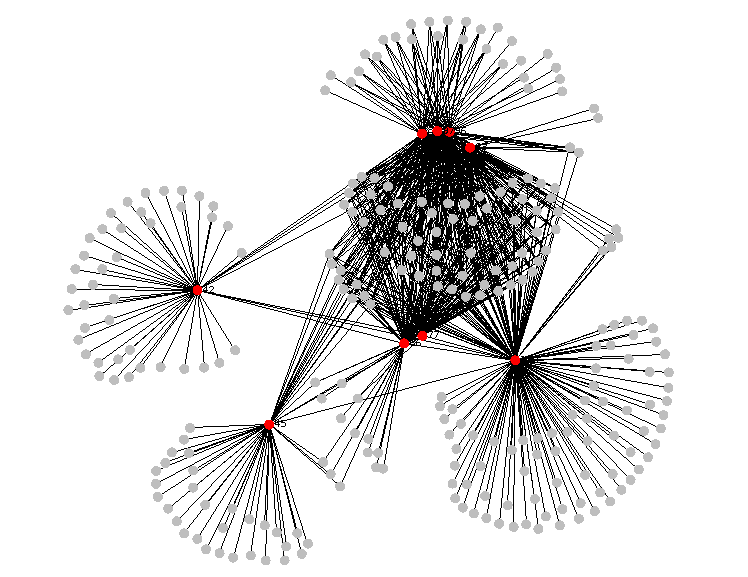
\includegraphics[scale=0.3]{web-graph.png}
\caption{Snapshot of the generated Web Graph}
\label{fig:web-graph}
\end{figure}

We then tried to build the Web graph using above web graph stream and Apache Spark's GraphX framework, however, we realized GraphX has no capability of working with streaming graphs. 

Then we moved on to Apache Flink, which is a relatively new streaming framework like Apache Spark, but not like Spark which is not truly real-time, but micro-batching based; Apache Flink as gained a lot of attention recently in the developer and research communities. Like Apache Spark, Flink is a streaming framework where we can plug different data streams and run different types of data analysis jobs on it. They too have a graph framework called Gelly, which run on top of Flink, like Apache Spark has GraphX.

However, same as GraphX, Gelly too is for static graphs. Fortunately, on of the researchers who as the same interest on graph streaming like us, has implemented a Gelly extension which can work with streaming graphs.

We then implemented a graph stream for Flink, using Twitter to build a social graph. Then we using the above extended Gelly framework, implemented the streaming graph. We then analysed the degree distributions of the graph time to time, as it grows. We realized there is a limitation in this scenario too. We can't dynamically submit any analysis on the building graph, but we have to pre define the analysis we need to do at the same time the graph start building. We communicated with the researcher who implemented the extension to Gelly about this and she confirmed it. 

Now, our next move is to take it further, try extend the Gelly to take analysis jobs on the run, while the graph keeps building. Furthermore, we are trying introduce graph sketching techniques and better partitioning techniques, then  analyse the performance gain.

\section{Research design with high-level diagrams}


\begin{figure}[H]
\centering
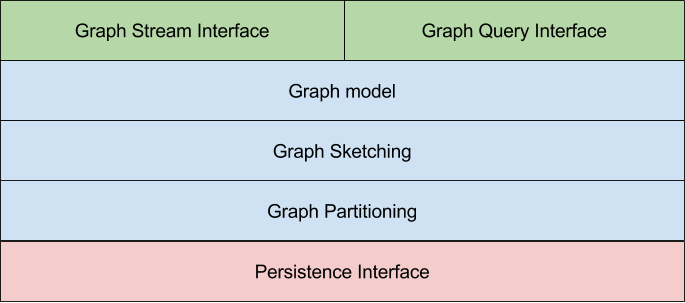
\includegraphics[scale=0.5]{intended-architecture.png}
\caption{Intended architecture of the platform}
\label{fig:intended-architecture}
\end{figure}

\subsection{Graph stream interface}
The users should be able to plug a stream of data to the systems, though a mapper which maps data into  edges and vertices and input to the graph model as a graph stream. 

\subsection{Graph model}
We can implement a graph in several ways, using linked list or a squire matrix are the popular options. We have to identify which method suits our needs and limitations. Some other options worth trying are non-square matrices which makes use of power low degree distribution of natural graphs. 

\subsection{Graph sketching}
Building a sketch of the graph makes us summarise the huge graph into a small model. There are many sketching techniques, some techniques limits the model for specific types of queries. We have to investigate good sketching techniques which does not limits us, and which suits well with the graph model ( linked list, squire matrix or non-square matrices ) we use and graph partitioning techniques we use. Figure \ref{fig:graph-sketching} shows how we can apply TCM \cite{TCM} model to sketch  graph. 

\begin{figure}[H]
\centering
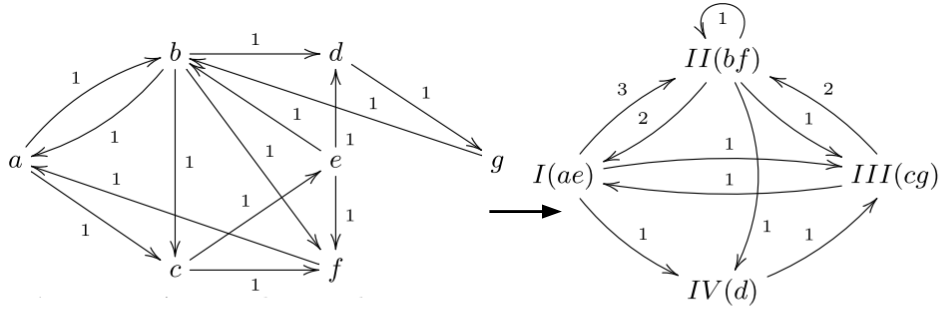
\includegraphics[scale=0.3]{graph-sketching.png}
\caption{Converting a graph into a TCM sketch}
\label{fig:graph-sketching}
\end{figure}

\subsection{Graph partitioning}
Partitioning depends on the above two factors, how we model the graph and how we sketch the graph. We have to find the best ways to minimize inter partition communication in order to obtain higher performance.

\subsection{Persistence interface}
We have to persist the data onto a storage and this should  be some persistence method which is familiar to the users. We could write to a Hadoop HDFS or to a database like Apache Cassandra.

\clearpage
\section{Literature Review}

We see several systems developed to cater the need of graphs related problems.

Apache Spark and its graph abstraction package GraphX\cite{GraphX} has gained lot of attention in the developer community for their graph based computational needs recently. GraphX also uses Pregel, but its own optimized variant of Pregel, in its underneath implementation.

And these systems uses different graph partitioning techniques. These techniques are base on various assumptions and have some limitations in some situations. There have been several researches done very recently and several papers published on the research problem on how to achieve better performance and how to avoid these limitations. 

\subsection{Static graphs}

\subsubsection{Pregel}

Pregel\cite{Pregel} graph framework was introduced for graph-parallel computations, where the computation is expressed as a sequence of steps, called 'supersteps'. In each step, a vertex receives a message from the previous step, changes its state and pass the message to the other vertices. Since Pregel is a synchronous system, it updates all parameters of vertices in parallel using values from the previous step as input. Partitioning of the graph is done by simply using a hash function on vertex ID. 

\subsubsection{GraphLab}

Then GraphLab\cite{Graphlab} \cite{DistributedGraphLab} was introduced for dynamic and asynchronous graph-parallel computation. GraphLab consists of a Data Graph which holds the program state, an Update Function, which is a stateless procedure, that updates the Data Graph in small chunks called Scopes and a Sync Function which concurrently maintains global aggregates. Different hash functions can be used to partition the graph. 

\subsubsection{DistributedGraphLab}

The Distributed GraphLab \cite{DistributedGraphLab} was to extend the GraphLab to fit to distributed environment.  

\subsubsection{Giraph}
Apache Giraph is one such graph processing system that is used at Facebook to analyse the social graph formed by users and their connections. It is an open-source implementation of Google’s Pregel\cite{Pregel} graph processing architecture. 

\subsubsection{Giraph++}
Giraph++\cite{GiraphPlusPlus} is an improved version of Apache Giraph, which is graph centric rather vertex centric. Main difference between Giraph and Giraph++ is, in Giraph++, the programmer can access the whole sub-graph in a partition, rather one vertex at a time. In Giraph++ each partition contains a set of vertices and all their outgoing edges. Each vertex is uniquely identified by an ID, and a partitioner decides which partition a vertex belongs to based on its ID. The partitioner is also used to route messages for a vertex correctly to its partition. The default partitioner is a hash function on the vertex ID.

\subsection{Streaming graphs}

\subsubsection{S-PowerGraph}

S-PowerGraph\cite{S-PowerGraph} discuss several methods as 'Degree', a greedy procedure which makes use of the in-degree distribution and 'DegreeIO' which tries to meet the challenge that both indegree and outdegree of natural graphs are skewed.

S-PowerGraph firstly suggests the Grid-based Constrained Random Vertex-cut algorithm of GraphBuilder\cite{Graphbuilder}  could be altered for streaming graph partitioning. In this method, a vertex is mapped into a shard which accommodates a constrained set of partitions. Then, the partition a vertex to be assigned will be chosen from the constrained set randomly. The edge e is assigned to P\textsubscript{idx} where idx is decided by idx = GridHash(e), the hash function implemented in GraphBuilder.

Then the S-PowerGraph discuss about an enhanced version of the greedy algorithm proposed in PowerGraph\cite{PowerGraph}. As the greedy algorithm in PowerGraph could lead to some unbalanced partitions in some cases, they introduce Balance(PowerGraph) where Balance() is a constraint to avoid the imbalance. 

\subsubsection{Apache Flink Gelly}
Apache Flink is a data stream processing framework and Flink's graph framework is Gelly. However, Gelly is only for static graphs. However, this \cite{Kalavri} is a research on how to extend to Gelly to support streaming. They have used Flink's shared states to continue the graph across iterations of the stream. 

\subsection{Graph partitioning}
\subsubsection{Fennel}

Fennel \cite{Fennel} is a one pass streaming graph partitioning technique which outperforms the de-facto standard offline software METIS on numerous real-world graphs, like Twitter graph with more than 1.4 billion of edges, which outputs balanced partitions.

\subsubsection{Linear Embedding}

"Distributed Balanced Partitioning via Linear Embedding"\cite{Linear Embedding} discusses a method researchers at Google have tried and tested with Google services. "Linear Embedding" is a balanced partitioning problem where the goal is to partition the vertices of a given graph into k parts so as to minimize the total cut size. Linear Embedding method first embeds nodes of the graph onto a line, then attempt to improve the ordering mainly by swapping vertices in a semi local manner and finally accommodate a post-processing method to improve the cut-size.

They discuss several different methods for each different step and compare the outcome performances for each combination. For embedding nodes onto a line,  they accommodate random mapping, Hilbert curve mapping when geographic/geometric information is available, and Affinity-based mapping which takes into account the affinity of vertices by grouping vertices that are closely connected, hence building a tree of these connections.

Once the linear embedding is done, the next step is to  improve ordering using semi local moves. One method is using Minimum Linear Arrangement (MinLA)\cite{MinLA} and the other is Rank Swap which depends on the pre chosen cut boundaries, the number of final partitions k. Finally they accommodate a post-processing method like dynamic programming to adjust the cut sizes.

\subsection{Graph sketching}
\subsubsection{TCM}
Sketching is process where we summarize a huge graph into a smaller graph, but we loose some data. Therefore we have to use different sketches for different types of queries. However, TCM is a research carried out for sketching which we can use for every types of queries. It uses hash buckets for sketching, and it not only sketch the edges, but also paths.

\subsection{Graph databases}

\subsubsection{Titan}
Titan is a distributed graph database engine build on top of Cassandra as the underlying data storage, but which now supports other data storage systems like HBase and BerkeleyDB. Titan natively supports the Gremlin Server component of the TinkerPop stack. Titan’s storage model is an adjacency list in a column family where row key is vertex id. Titan maintains indexes in a separate column family and one nice feature of Titan is we can accommodate third party tools like Elasticsearch, Lucene, etc for indexing.


\end{document}   
